\documentclass[11pt]{article}
\title{Lenses}
\author{https://github.com/heptagons/lenses}
\date{2023/12/31}

\usepackage{graphicx}

\usepackage[margin=0.75in]{geometry}
\usepackage{float} % {figure}{H}
\usepackage{amsmath} % \dfrac


%\usepackage{amssymb}
%\usepackage{subcaption}

\def\mathbi#1{\textbf{\em #1}}

\begin{document}

\maketitle
\begin{abstract}
Lenses are equilateral hexagons resembling concave and convex optical lenses. Lenses consecutive six internal angles are $(\theta_1,\theta_2,\theta_3,\theta_1,\theta_2,\theta_3)$ where $\theta_1=X\theta_0$, $\theta_2=Y\theta_0$, and $\theta_3=Z\theta_0$ where $\theta_0 = 2\pi/S$ is the base angle of symmetry $S = X + Y + Z$.
\end{abstract}

\section{Lenses}

\section{Symmetry $5$}

Symmetry $5$ uses as base the angle $\beta = \dfrac{2\pi}5$ and produces the two rhombi $(\mathbi{b},\mathbi{c})$ and the two lenses $(\mathbi{B},\mathbi{C})$.


\subsection{Rhombi (\mathbi{b},\mathbi{c})}

\begin{figure}[H]
\centering
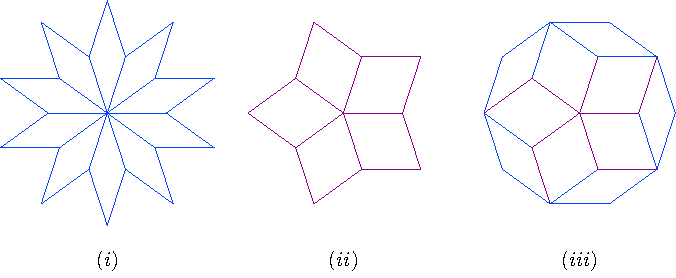
\includegraphics[scale=1.1]{bc/rhombi}
\caption{Rhombi $(\mathbi{b},\mathbi{c})$.}
\label{fig:bc-rhombi}
\end{figure}

\begin{table}[H]
\begin{center}
\begin{tabular}{|c|c c|}
\hline
Rhombus & $\theta_1$ & $\theta_2$ \\ %[1ex]
\hline\
$\mathbi{b}$ & $\beta/2$ & $4\beta/2$ \\[0.5ex] \hline
%& \\[-1ex]
$\mathbi{c}$ & $2\beta/2$ & $3\beta/2$ \\[0.5ex] \hline
%\hline
%\hline
\end{tabular}
\caption{Rhombi $(\mathbi{b},\mathbi{c})$ internal angles $\theta_1 + \theta_2 = \pi$ where $\beta = 2\pi/5$.} 
\label{tbl:bc-angles}
\end{center}
\end{table}

Figure \ref{fig:bc-rhombi} show rhombi $(\mathbi{b},\mathbi{c})$. 
From the figures we calculate the areas adding the rhombi:
Star $(i)$ area is $10\mathbi{b}$, star $(ii)$ area is $5\mathbi{c}$ and 
regular decagon $(iii)$ area is $5\mathbi{b} + 5\mathbi{c}$. Table \ref {tbl:bc-angles} show the rhombi angles.

\begin{figure}[H]
\centering
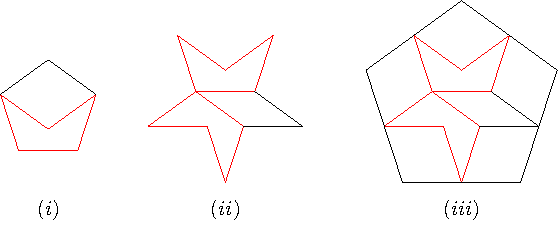
\includegraphics[scale=1.1]{bc/penta}
\caption{Pentagon $\{5/1\}$ and pentagram $\{5/2\}$.}
\label{fig:bc-penta}
\end{figure}

Figure \ref{fig:bc-penta} show regular pentagon and pentagram dissected with rhombi $(\mathbi{b},\mathbi{c})$ and a concave pentagon (in gray). We calculate the areas of the regular pentagon $P_1$ at $(i)$ and pentagram $P_2$ at $(ii)$ in function of rhombi $(\mathbi{b},\mathbi{c})$. Let $x$ be the concave pentagon area. From the figures we note pentagon $P_4$ at $(iii)$ is double the side and then four times the area of pentagon $P_1$. From the figures we note the area of $P_1$ is $ \mathbi{c} + x$ and the area of $P_4$ is $\mathbi{b} + 5\mathbi{c} + 2x$, so we compare the pentagons and solve for $x$ to get:
\begin{align}
4P_1 &= P_4 \nonumber\\
4(\mathbi{c} + x) &= \mathbi{b} + 5\mathbi{c} + 2x\nonumber\\
x &= \frac{\mathbi{b} + \mathbi{c}}2
\end{align}

We use $x$ to get the areas of pentagon and pentagram:
\begin{align}
P_1 &= \mathbi{c} + x
 =  \mathbi{c} + \frac{\mathbi{b} + \mathbi{c}}2
 = \frac{\mathbi{b} + 3\mathbi{c}}2 \\
P_2 &= \mathbi{b} + 2x
 =  \mathbi{b} + \frac{2(\mathbi{b} + \mathbi{c})}2
 = 2\mathbi{b} + \mathbi{c}
\end{align}

\subsection{Lenses (\mathbi{B},\mathbi{C})}

\begin{figure}[H]
\centering
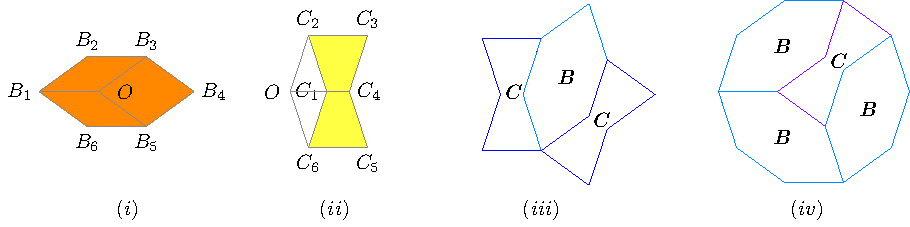
\includegraphics[scale=1.1]{bc/hexagons}
\caption{Lenses (\mathbi{B}, \mathbi{C}).}
\label{fig:bc-hexagons}
\end{figure}

\begin{table}[H]
\begin{center}
\begin{tabular}{|c|c c c|}
\hline
Rhombus & $\theta_1$ & $\theta_2$ & $\theta_3$ \\ %[1ex]
\hline\
$\mathbi{B}$ & $\beta$ & $2\beta$ & $2\beta$ \\[0.5ex] \hline
%& \\[-1ex]
$\mathbi{C}$ & $\beta$ & $\beta$ & $3\beta$ \\[0.5ex] \hline
%\hline
%\hline
\end{tabular}
\caption{Lenses $(\mathbi{B},\mathbi{C})$ internal angles $\theta_1+\theta_2+\theta_3 = 2\pi$ where $\beta = 2\pi/5$.} 
\label{tbl:bc-lenses-angles}
\end{center}
\end{table}


Figure \ref{fig:bc-hexagons} show lenses $(\mathbi{B},\mathbi{C})$.
Figure $(i)$ show the lense $\mathbi{B}$ with perimeter $\overline{B_1...B_6}$ is formed adding two rhombi $\mathbi{b}$ and adding one rhombus $\mathbi{c}$ so its area is $2\mathbi{b} + \mathbi{c}$.
Figure $(ii)$ show the lense $\mathbi{C}$ with perimeter $\overline{C_1...C_6}$ is formed adding two rhombi $\mathbi{c}$ and substracting one rhombus $\mathbi{b}$ so its area is $2\mathbi{c} - \mathbi{b}$.
From the figures we see the area of star $(iii)$ is $\mathbi{B} + 2\mathbi{C} = 5\mathbi{c}$
and the area of regular decagon $(iv)$ is $3\mathbi{B} + \mathbi{C} = 5\mathbi{b} + 5\mathbi{c}$.

\section{Symmetry $7$}

Symmetry $7$ uses as base the angle $\gamma = \dfrac{2\pi}7$ and produces the three rhombi $(\mathbi{d},\mathbi{f},\mathbi{e})$ and the three lenses $(\mathbi{D},\mathbi{E},\mathbi{F})$.

\subsection{Rhombi $(\mathbi{d},\mathbi{e},\mathbi{f})$}

\begin{figure}[H]
\centering
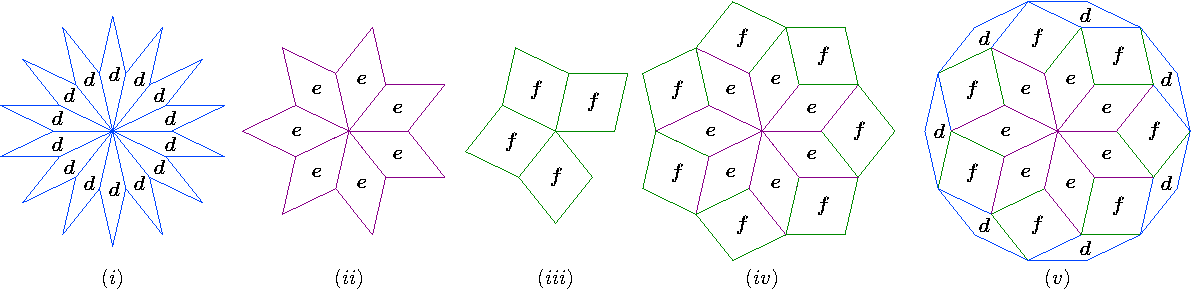
\includegraphics[scale=0.9]{def/rhombi}
\caption{Rhombi $(\mathbi{d},\mathbi{e},\mathbi{f})$.}
\label{fig:def-rhombi}
\end{figure}

\begin{table}[H]
\begin{center}
\begin{tabular}{|c|c c|}
\hline
Rhombus & $\theta_1$ & $\theta_2$ \\ %[1ex]
\hline\
$\mathbi{d}$ & $\gamma/2$ & $6\gamma/2$ \\[0.5ex] \hline
$\mathbi{e}$ & $2\gamma/2$ & $5\gamma/2$ \\[0.5ex] \hline
$\mathbi{f}$ & $3\gamma/2$ & $4\gamma/2$ \\[0.5ex] \hline
%\hline
%\hline
\end{tabular}
\caption{Rhombi $(\mathbi{d},\mathbi{e},\mathbi{f})$ internal angles $\theta_1 + \theta_2 = \pi$ where $\gamma = 2\pi/7$.} 
\label{tbl:def-angles}
\end{center}
\end{table}

Figure \ref{fig:def-rhombi} show rhombi $(\mathbi{d},\mathbi{e},\mathbi{f})$. 
Inspecting the figures we get the areas simply adding the rhombi:
Star $(i)$ area is $14\mathbi{d}$, star $(ii)$ area is $7\mathbi{e}$. The star $(iv)$ area is $7(\mathbi{e} + \mathbi{f})$ and the regular 14-gon area is $7(\mathbi{d} + \mathbi{e} + \mathbi{f})$. Table \ref {tbl:def-angles} show the symmetry 7 rhombi angles.


\begin{figure}[H]
\centering
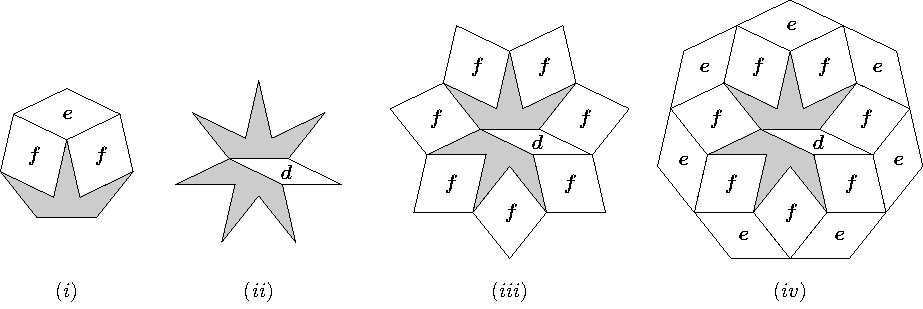
\includegraphics[scale=1.1]{def/hepta}
\caption{Heptagon $\{7/1\}$ at $(i)$ and heptagrams $\{7/2\}$ at $(ii)$ and $\{7/3\}$ at $(iii)$.}
\label{fig:def-hepta}
\end{figure}

Figure \ref{fig:def-hepta} show regular heptagon and heptagrams dissected with rhombi $(\mathbi{c},\mathbi{d},\mathbi{e})$ and with one equilateral concave heptagon (in gray). Let $\mathbi{x}$ the area of such gray piece. By inspection the area of regular heptagon at $(i)$ is $H_1 = \mathbi{e} + 2\mathbi{f} + \mathbi{x}$ while the area of regular heptagon at $(iv)$ is $H_2 = \mathbi{d} + 7(\mathbi{e}+\mathbi{f}) + 2\mathbi{x}$. Since the side of $H_2$ is the double of $H_1$ its area is four times so we can get the value of $\mathbi{x}$:
\begin{align}
4H_1 &= H_2 \nonumber\\
4(\mathbi{e} + 2\mathbi{f} + \mathbi{x}) &= \mathbi{d} + 7(\mathbi{e}+\mathbi{f}) + 2\mathbi{x} \nonumber\\
\mathbi{x} &= \frac{\mathbi{d} + 3\mathbi{e} - \mathbi{f}}2
\end{align}

We use the value of $\mathbi{x}$ to calculate the areas of heptagon $(i)$ and heptagrams $(ii)$ and $(iii)$ in function of $(\mathbi{d},\mathbi{e},\mathbi{f})$:
\begin{align}
A\{7/1\} &= \mathbi{e} + 2\mathbi{f} + \mathbi{x} \nonumber\\
    &= \frac{\mathbi{d} + 5\mathbi{e} + 3\mathbi{f}}2 \\
A\{7/2\} &= \mathbi{d} + 2\mathbi{x} \nonumber\\
 &= 2\mathbi{d} + 3\mathbi{e} - \mathbi{f} \\
A\{7/3\} &= A\{7/2\} + 7\mathbi{f} \nonumber\\
 &= 2\mathbi{d} + 3\mathbi{e} + 6\mathbi{f}
\end{align}



\end{document}
